\documentclass[landscape,footrule]{foils}
\usepackage[lecture-serie]{foiltex-extra}
\usepackage{color}
\usepackage{crysymb}
\usepackage[draft]{crygame}
\usepackage{crypto-ii}
\usepackage{graphics}
\usepackage[pdftex]{graphicx} 


\newcommand{\lecture}{Public Key Cryptosystems}
\newcommand{\lserie}{MTAT.07.003 Cryptology II}
\newcommand{\ldate}{19 March, 2010}
\newcommand{\lauthor}{Sven Laur}
\newcommand{\linst}{University of Tartu}
\graphicspath{{./illustrations/}}


\newcommand{\lastline}{\vspace*{-2ex}}
\newcommand{\spreadappart}{\vspace*{\fill}}


\renewcommand{\SK}{{\red{\mathsf{sk}}}}
\renewcommand{\PK}{{\blue{\mathsf{pk}}}}
\newcommand{\GUESS}{\green{\mathsf{guess}}}

\begin{document}

\titlefoil
\middlefoil{Formal Syntax}


\foilhead[-1.5cm]{Public key cryptosystem}

\illustration[scale=0.8, angle=-90, clip, trim=1.5cm 1.5cm 11.6cm 1.5cm]{passive-attack-ii.eps} 
\vspace*{1ex}
\begin{triangles}
\item A randomised \emph{key generation algorithm} outputs a
  \emph{secret key} $\SK$ and a \emph{public key} $\PK$. A public
  key gives ability to encrypt messages.
\item A randomised \emph{encryption algorithm}
  $\ENC_\PK:\MSPACE\to\CSPACE$ takes in a \emph{plaintext} and
  outputs a corresponding \emph{ciphertext}.
\item A \emph{decryption algorithm}
  $\DEC_\SK:\CSPACE\to\MSPACE\cup\set{\bot}$ recovers the plaintext or
  a special abort symbol $\bot$ to indicate invalid ciphertexts.
\end{triangles}





\foilhead[-1cm]{Example. RSA-1024 cryptosystem}

\textbf{Key generation $\GEN$:}
\begin{enumerate}
\item Choose uniformly $512$-bit prime numbers $p$ and $q$.
\item Compute $N=p\cdot q$ and $\phi(N)=(p-1)(q-1)$.
\item Choose uniformly $e\gets\ZZ_{\phi(N)}^*$ and set $d=e^{-1}\mod \phi(N)$.
\item Output $\SK=(p,q,e,d)$ and $\PK=(N,e)$.
\end{enumerate}

\vskip 1cm
\textbf{Encryption and decryption:}

\begin{align*}
 \MSPACE=\ZZ_N,\quad \CSPACE=&\ZZ_N,\quad \RSPACE=\emptyset\\
\ENC_\PK(m)=m^{\blue{e}}\mod N\quad&\quad\DEC_\SK(c)=c^{\red{d}}\mod N\enspace.
\end{align*}



\middlefoil{Semantic Security}

 
\foilhead[-1cm]{IND-CPA security}\enlargethispage{2cm}

As a potential adversary $\AD$ can influence which messages are
encrypted, we must model the corresponding effects in our attack
model.  A cryptosystem $(\GEN,\ENC,\DEC)$ is
\emph{$(t,\varepsilon)$-IND-CPA secure} if for all $t$-time
adversaries $\AD$:
\begin{align*}
  \advINDCPAXX{}{\AD}
   &=\bigl|\pr{\GAME_0^\AD=1}-\pr{\GAME_1^\AD=1}\bigr|\leq \varepsilon\enspace,
\end{align*}
where the security games are defined as follows \vspace*{-2ex}
\begin{align*}
  \begin{game}{\GAME_0^\AD}
    &(\SK,\PK)\gets\GEN\\
    &(m_0,m_1)\gets\AD(\PK)\\
    &\RETURN \AD(\enc{m_0})
  \end{game}
  \qquad\qquad
  \begin{game}{\GAME_1^\AD}
    &(\SK,\PK)\gets\GEN\\
    &(m_0,m_1)\gets\AD(\PK)\\
    &\RETURN \AD(\enc{m_1})
  \end{game}
\end{align*}



\foilhead[-1cm]{Semantic security against adaptive influence}

\illustration[scale=0.82, angle=-90, clip, trim=3.5cm 2.5cm 4.0cm 2.5cm]{semantic-security.eps}


\foilhead[-1cm]{Formal definition}\enlargethispage{2cm}

Consider following games:\vspace*{-3ex}
\begin{align*}
  \begin{game}{\GAME_0^\AD}
    &(\SK,\PK)\gets\GEN\\
    &\MSPACE_0\gets\AD(\PK)\\
    &m\gets\MSPACE_0\\
    &c\gets\ENC_\PK(m)\\
    &\RETURN [g(m)\iseq \AD(c)]
  \end{game}
  \qquad\qquad
  \begin{game}{\GAME_1^\AD}
    &(\SK,\PK)\gets\GEN\\
    &\MSPACE_0\gets\AD(\PK)\\
    &m\gets\MSPACE_0,\orangecommand{\smash{\overline{m}\gets\MSPACE_0}}\\
    &\orangecommand{\smash{\overline{c}\gets\ENC_\PK(\overline{m})}}\\
    &\RETURN [g(m)\iseq \orangecommand{\smash{\AD(\overline{c})}}]
  \end{game}
\end{align*}\vspace{-3ex}\\
The true guessing advantage is
\begin{align*}
 \advSemXX{g}{\AD}=\pr{\smash{\GAME_0^\AD=1}}-\pr{\smash{\GAME_1^\AD=1}}\enspace.
\end{align*}





\foilhead[-1cm]{IND-CPA $\Rightarrow$ SEM-CPA}

\textbf{Theorem}. Assume that $g$ is a $t_g$-time function and it is
always possible to obtain a sample from $\MSPACE_0$ in time
$t_m$. Now if the cryptosystem is $(t,\varepsilon)$-IND-CPA secure,
then for all $(t-t_g-2t_m)$-time adversaries $\AD$:
\begin{align*}
  \advSemXX{g}{\AD}\leq\varepsilon\enspace.
\end{align*}
\vskip 1.5cm
Note that
\begin{triangles}
\item The function $g$ might be randomised.
\item The function $g$ must be efficiently computable.
\item The distribution $\MSPACE_0$ must be efficiently samplable.
\end{triangles}



\middlefoil{An Example of IND-CPA Secure\vspace*{1ex}\\ Cryptosystem}

\foilhead[-1cm]{ElGamal cryptosystem}



Combine the Diffie-Hellman key exchange protocol
\begin{align*}
 &\textbf{Alice} && &\textbf{Bob}\\
 & \textcolor{red}{x}\gets\ZZ_{\abs{\GG}}& &\xrightarrow{y=g^x} && \textcolor{red}{k}\gets\ZZ_{\abs{\GG}}\\
 && &\xleftarrow{\ g^k\ }\\
 &\textcolor{red}{g^{xk}}=(g^k)^{\textcolor{red}{x}} && &\textcolor{red}{g^{xk}}=(g^x)^{\textcolor{red}{k}}
\end{align*}
with one-time pad by multiplication using in $\GG=\langle g\rangle$ as
encoding rule
\begin{align*}
  \enc{m}=(g^k,m{}\cdot \textcolor{red}{g^{xk}})=(g^k,m{}\cdot y^k) \qquad 
  \text{for all elements } m\in \GG
\end{align*}
with a public key $\PK=y=g^{\textcolor{red}{x}}$ and a secret key $\SK=\textcolor{red}{x}$.
  


\foilhead[-1cm]{Decisional Diffie-Hellman Assumption (DDH)}

\textbf{Definition.} We say that a $q$-element multiplicative group
$\GG$ is $(t,\varepsilon)$-Decisional Diffie-Hellman group if for all
$t$-time adversaries $\AD$:
\begin{align*}
  \advDDHXX{\GG}{\AD}=\abs{\pr{\smash{\GAME_0^\AD=1}}-\pr{\smash{\GAME_1^\AD=1}}}\leq\varepsilon
\end{align*}
where the security games are defined as follows
\begin{align*}
  \begin{game}{\GAME_0^\AD}
    &x,k\gets\ZZ_q\\
    &\RETURN \AD(g,g^x,g^k,g^{xk})
  \end{game}
  \qquad\qquad 
  \begin{game}{\GAME_1^\AD}
    &x,k,c\gets\ZZ_q\\
    &\RETURN \AD(g,g^x,g^k,g^{c})
  \end{game}
\end{align*}

 
The Diffie-Hellman key exchange protocol is secure under the DDH
assumption, as an attacker cannot distinguish values $g^{xk}$
and $g^c$. \lastline


\foilhead[-1cm]{DDH $\Rightarrow$  IND-CPA}

\textbf{Theorem}. Let $\GG$ be a $(t,\varepsilon)$-DDH group. Then the
corresponding instantiation of the ElGamal cryptosystem is
$(t,2\varepsilon)$-IND-CPA secure.


Let $\ADB$ be good against IND-CPA games. Then we can consider the
following algorithm $\AD$: 
\begin{enumerate}
\item Given $(g,g^x,g^k,z)$, set $\PK=g^x$ and
  $(m_0,m_1)\gets\ADB(\PK)$.
  \item Toss a fair coin $b\gets\set{0,1}$ and set $c=(g^k,m_bz)$.
  \item If $b\iseq \AD(c)$ return $1$ else output $0$.  
\end{enumerate}

\vskip 1cm
We argue that this is a good strategy to win the DDH game:
\begin{bullets}
 \item In the game $\GAME_0$, we simulate the bit guessing game. 
 \item In the game $\GAME_1$, the guess $\GUESS$ is independent form $b$. 
\end{bullets}

\foilhead[-1cm]{Hybrid encryption}

Assume that $(\GEN,\ENC,\DEC)$ is a IND-CPA secure public key
cryptosystem and $(\GEN^\circ,\ENC^\circ,\DEC^\circ)$ is a IND-CPA
secure symmetric key cryptosystem. Then we can construct a hybrid
IND-CPA secure cryptosystem.

\textbf{Key generation.} Output the original secret and public key
$(\SK,\PK)\gets\GEN$.

\textbf{Encryption.} For $m\in\MSPACE^\circ$ generate a session key
$\SK^\circ\gets\GEN^\circ$  and compute
\begin{align*}
  \ENC_\PK^*(m)=(\enc{\SK^\circ},\ENC_{\SK^\circ}^\circ(m))
\end{align*}
\textbf{Decryption.} Given $(c_1,c_2)$ compute $\SK^\circ\gets\dec{c_1}$ and
output $\DEC_{\SK^\circ}^\circ(c_2)$.

\bigskip

\textbf{Theorem.} The hybrid encryption is
$(t,2\varepsilon_1+\varepsilon_2)$-IND-CPA secure if the public key
cryptosystem is $(t,\varepsilon_1)$-IND-CPA secure and the symmetric
key cryptosystem is $(t,\varepsilon_2)$-IND-CPA secure.\lastline


\foilhead[-1cm]{Corresponding proof}

\begin{small}
\begin{align*}
  \begin{game}{\GAME_0^\AD}
    &(\SK,\PK)\gets\GEN\\
    &(m_0,m_1)\gets\AD(\PK)\\
    &\SK^\circ\gets\GEN^\circ\\
    &\overline{\SK}^\circ\gets\GEN^\circ\\
    &\orangecommand{\smash{c_1\gets\ENC_\PK(\SK^\circ)}}\\
    &c_2\gets\ENC_{\SK^\circ}^\circ(m_0)\\
    &\RETURN \AD(c_1,c_2)
  \end{game}
  \Redarrow{\text{IND-CPA}}{\varepsilon_1}
  \begin{game}{\GAME_2^\AD}
    &(\SK,\PK)\gets\GEN\\
    &(m_0,m_1)\gets\AD(\PK)\\
    &\SK^\circ\gets\GEN^\circ\\
    &\overline{\SK}^\circ\gets\GEN^\circ\\
    &\orangecommand{\smash{c_1\gets\ENC_\PK(\overline{\SK}^\circ)}}\\
    &\orangecommand{\smash{c_2\gets\ENC_{\SK^\circ}^\circ(m_0)}}\\
    &\RETURN \AD(c_1,c_2)
  \end{game}
  \Redarrow{\text{IND-CPA}}{\varepsilon_2}
  \begin{game}{\GAME_3^\AD}
    &(\SK,\PK)\gets\GEN\\
    &(m_0,m_1)\gets\AD(\PK)\\
    &\SK^\circ\gets\GEN^\circ\\
    &\overline{\SK}^\circ\gets\GEN^\circ\\
    &c_1\gets\ENC_\PK(\overline{\SK}^\circ)\\
    &\orangecommand{\smash{c_2\gets\ENC_{\SK^\circ}^\circ(m_1)}}\\
    &\RETURN \AD(c_1,c_2)
  \end{game}
 \qquad
\end{align*}
\end{small}


\middlefoil{Ciphertext modification attacks}

\foilhead[-2cm]{Symmetric key cryptosystem}

\illustration[scale=0.8, angle=-90, clip, trim=1.5cm 1.5cm 11.6cm 1.5cm]{active-attack-i.eps}
\vspace*{1ex}
\begin{triangles}
\item A malicious participant may control the communication network
  and alter the ciphertexts to bypass various security checks.
\item A malicious participant may interact with a key holder and use
  him or her as an \emph{encryption} or \emph{decryption} oracle.
\item A non-malleable encryption  detects modifications in ciphertexts
  (\emph{authenticated encryption}) or assures that $m{}$ and
  $\overline{m{}}$ are unrelated.
\end{triangles}



\foilhead[-2cm]{Public key cryptosystem}

\illustration[scale=0.8, angle=-90, clip, trim=1.5cm 1.5cm 11.6cm 1.5cm]{active-attack-ii.eps}
\vspace*{1ex}
\begin{triangles}
\item Active attacks are similar for public key cryptosystems. Except
  there is no need for encryption oracle, since the adversary knows
  the public key.
\item Common cryptosystems detect tampered ciphertexts with
  high probability and thus the adversary cannot use the decryption
  oracle for useful tasks.
\end{triangles}

\foilhead[-1cm]{Homological classification}

\begin{center}
  \includegraphics[scale=0.82, angle=-90, clip, trim=3.5cm 2.5cm 11.1cm
  2.5cm]{homological-classification.eps}
\end{center}

The figure above depicts the relations among various security
properties of public key cryptosystems. In practise one normally needs: 
\begin{triangles}
  \item semantic security that follows IND-CPA security,
  \item safety against improper usage that follows form IND-CCA1 security, 
  \item non-malleability of ciphertexts that follows form NM-CPA security.
\end{triangles}



\foilhead[-1cm]{Safety against improper usage}

Cleverly crafted ciphertexts or ciphertext-like messages may provide
relevant information about the secret key or even reveal the secret key.

Such attacks naturally occur in:
\begin{triangles}
  \item smart card cracking (Satellite TV, TPM-modules, ID cards)
  \item authentication protocols (challenge-response protocols) 
  \item side-channel attacks (timing information, encryption failures)
\end{triangles}

\vskip 2ex
\textbf{Minimal security level:}
\begin{triangles}
\item Attacks reveal information only about currently known
  ciphertexts.
\end{triangles}

\vskip 2ex
\textbf{Affected cryptosystems:}
\begin{itemize}
\item Rabin cryptosystem, some versions of NTRU cryptosystem, etc.
\end{itemize}


\foilhead[-1cm]{IND-CCA1 security}\enlargethispage{1cm}

A cryptosystem is \emph{$(t,\varepsilon)$-IND-CCA1 secure} if for all
$t$-time adversaries $\AD$:
\begin{align*}
  \advINDCCAIXX{}{\AD}
   &=\bigl|\pr{\GAME_0^\AD=1}-\pr{\GAME_1^\AD=1}\bigr|\leq \varepsilon\enspace,
\end{align*}
where the security games are defined as follows \vspace*{-2ex}
\begin{align*}
  \begin{game}{\GAME_0^\AD}
    &(\SK,\PK)\gets\GEN\\
    &(m_0,m_1)\gets\AD^{\ORA_1(\cdot)}(\PK)\\
    &\RETURN \AD(\enc{m_0})
  \end{game}
  \qquad\qquad
  \begin{game}{\GAME_1^\AD}
    &(\SK,\PK)\gets\GEN\\
    &(m_0,m_1)\gets\AD^{\ORA_1(\cdot)}(\PK)\\
    &\RETURN \AD(\enc{m_1})
  \end{game}
\end{align*}
and the oracle $\ORA_1$ serves decryption queries, i.e., $\ORA_1(c)=\dec{c}$.
  


\foilhead[-1cm]{Rabin cryptosystem}

\textbf{Key generation $\GEN$:}
\begin{enumerate}
\item Choose uniformly $512$-bit prime numbers $p$ and $q$.
\item Compute $N=p\cdot q$ and $\phi(N)=(p-1)(q-1)$.
\item Output $\SK=(p,q)$ and $\PK=N$.
\end{enumerate}

\vskip 1cm
\textbf{Encryption and decryption:}

\begin{align*}
 \MSPACE=\ZZ_N,\quad \CSPACE=&\ZZ_N,\quad \RSPACE=\emptyset\\
\ENC_\PK(m)=m^2\mod N\quad&\quad\DEC_\SK(c)=\sqrt{c}\mod N\enspace.
\end{align*}

\foilhead[-1cm]{Lunchtime attack}

\begin{enumerate}
\item Choose $x\gets \ZZ_N^*$ and set $c\gets x^2\mod N$.
\item Compute decryption $\overline{x}\gets\ORA_1(c)$.
\item If $\overline{x}\neq \pm x$ then
  \begin{itemize}
  \item Compute nontrivial square root $\xi=\overline{x}\cdot x^{-1}\mod N$
  \item Compute a nontrivial factors $p\gets\gcd(N,\xi+1)$ and $q=N/p$.
  \item Output a secret key $\SK=(p,q)$.
  \end{itemize}\vspace*{1ex}
\item Continue from Step 1. 
\end{enumerate}

\vskip 1cm
\textbf{Efficiency analysis}
\begin{itemize}
  \item Each iteration fails with probability $\frac{1}{2}$.
  \item With $80$ decryption queries the failure probability is $2^{-80}$. 
\end{itemize}

\foilhead[-1cm]{IND-CCA2 security}\enlargethispage{1cm}

A cryptosystem is \emph{$(t,\varepsilon)$-IND-CCA2 secure} if for all
$t$-time adversaries $\AD$:
\begin{align*}
  \advINDCCAIXX{}{\AD}
   &=\bigl|\pr{\GAME_0^\AD=1}-\pr{\GAME_1^\AD=1}\bigr|\leq \varepsilon\enspace,
\end{align*}
where the security games are defined as follows \vspace*{-2ex}
\begin{align*}
  \begin{game}{\GAME_0^\AD}
    &(\SK,\PK)\gets\GEN\\
    &(m_0,m_1)\gets\AD^{\ORA_1(\cdot)}(\PK)\\
    &\RETURN \AD^{\ORA_2(\cdot)}(\enc{m_0})
  \end{game}
  \qquad\qquad
  \begin{game}{\GAME_1^\AD}
    &(\SK,\PK)\gets\GEN\\
    &(m_0,m_1)\gets\AD^{\ORA_1(\cdot)}(\PK)\\
    &\RETURN \AD^{\ORA_2(\cdot)}(\enc{m_1})
  \end{game}
\end{align*}
and oracles $\ORA_1$ and $\ORA_2$ serve decryption queries,
i.e., $\ORA_1(c)=\dec{c}$ and $\ORA_2(c)=\dec{c}$ for all
non-challenge ciphertexts.



\foilhead[-1cm]{IND-CCA2 secure cryptosystems}

All known IND-CCA2 secure cryptosystems include a non-interactive
proof that the creator of the ciphertexts $c$ knows the corresponding
message $m$:

\begin{itemize}
\item the RSA-OAEP cryptosystem in the random oracle model,
  \item the Cramer-Shoup cryptosystem in standard model,
  \item the Kurosawa-Desmedt key encapsulation scheme.  
\end{itemize}


\middlefoil{Non-malleability}

\foilhead[-1cm]{NM-CPA security}
\begin{center}
 \includegraphics[scale=0.82, angle=-90, clip, trim=3.5cm 2.5cm 4.0cm 2.5cm]{non-malleability.eps}
\end{center}

\foilhead[-2.5cm]{Formal definition}\enlargethispage{1cm}

\begin{align*}
  \begin{game}{\GAME_0^\AD}
    &(\SK,\PK)\gets\GEN\\
    &\red{\MSPACE_0}\gets\AD(\PK)\\
    &m\gets\red{\MSPACE_0}\\
    &c\gets\ENC_\PK(m)\\
    &\pi(\cdot),\hat{c}_1,\ldots\hat{c}_n\gets\AD(c)\\
    &\IF c\in\set{\hat{c}_1,\ldots\hat{c}_n}\THEN \RETURN 0\\
    &\RETURN \pi(m,\dec{\hat{c}_1},\ldots)
  \end{game}
  \qquad\qquad
  \begin{game}{\GAME_1^\AD}
    &(\SK,\PK)\gets\GEN\\
    &\red{\MSPACE_0}\gets\AD(\PK)\\
    &m\gets\red{\MSPACE_0},\orangecommand{\smash{\overline{m}\gets\red{\MSPACE_0}}}\\
    &\orangecommand{\smash{\overline{c}\gets \ENC_\PK(\overline{m})}}\\
    & \pi(\cdot),\hat{c}_1,\ldots\hat{c}_n\gets{\smash{\AD(\overline{c})}}\\
    &\IF \overline{c}\in\set{\hat{c}_1,\ldots\hat{c}_n}\THEN \RETURN 0\\
    &\RETURN \pi(m,\dec{\hat{c}_1},\ldots) 
  \end{game}
\end{align*}\vspace{-3ex}\\
The true  advantage is\vspace{-1ex}
\begin{align*}
 \advNMCPAXX{}{\AD}=\abs{\pr{\smash{\GAME_0^\AD=1}}-\pr{\smash{\GAME_1^\AD=1}}}
\end{align*}



\foilhead[-1cm]{Homological classification}

\begin{center}
  \includegraphics[scale=0.82, angle=-90, clip, trim=3.5cm 2.5cm 11.1cm
  2.5cm]{homological-classification.eps}
\end{center}

Horizontal implications are trivial.
\begin{bullets}
 \item The adversary just gets more powerful in the row. 
\end{bullets}

Downwards implications are trivial.
\begin{bullets}
  \item A guess $\GUESS$ can be passed as a predicate $\pi(\cdot)\equiv 0$ and $\pi(\cdot)\equiv 1$. 
\end{bullets}


\foilhead[-1cm]{IND-CCA2 $\Rightarrow$ NM-CC2}

\textbf{Theorem}. Assume that $\pi(\cdot)$ is always a $t_\pi$-time
predicate and it is always possible to obtain a sample from $\MSPACE_0$
in time $t_m$. Now if the cryptosystem is $(t,\varepsilon)$-IND-CCA2
secure, then for all $(t-t_g-2t_m)$-time adversaries $\AD$:
\begin{align*}
  \advNMCCAIIXX{}{\AD}\leq\varepsilon\enspace.
\end{align*}
\vskip 1.0cm
Note that
\begin{triangles}
\item The predicate $\pi(\cdot)$ might be randomised.
\item The predicate $\pi(\cdot)$ might have variable number of
  arguments.
\item The predicate $\pi(\cdot)$ must be a computationally  efficient function.
\item The distribution $\MSPACE_0$ must be efficiently samplable.
\end{triangles}

\foilhead[-1cm]{The corresponding proof}

Let $\ADB$ be an adversary that is good in NM-CCA2 games. Then we can
emulate NM-CCA2 game given access to the decryption oracle $\ORA_2$:
\begin{enumerate}
  \item $\AD$ forwards $\PK$ to $\ADB$ who sends back a description of $\red{\MSPACE_0}$. 
  \item $\AD$ independently samples $m_0\gets\red{\MSPACE_0}$ and $m_1\gets\red{\MSPACE_0}$.
  \item $\AD$ forwards the challenge $\enc{m_b}$ to $\ADB$.
  \item $\ADB$ sends $\hat{c}_1,\ldots,\hat{c}_n$ and
    $\pi(\cdot)$ to $\AD$ who 
    \begin{itemize}
      \item uses $\ORA_2$ to recover $\dec{\hat{c}_1},\ldots,\dec{\hat{c}_n}$,
      \item outputs $\pi(m_0,\dec{\hat{c}_1},\ldots,\dec{\hat{c}_n})$ as the final output.
    \end{itemize}
\end{enumerate}

\vskip 0.75cm
\textbf{Running time}\vspace*{1ex} \\
The running time of $\AD$ is $t_b+t_g+2t_m$ where $t_b$ is the running
time of $\ADB$.

\foilhead[-1cm]{Further analysis by code rewriting}

For clarity, let $\BGAME_0$ and $\BGAME_1$ denote the IND-CCA2 security
games and $\GAME_0$ and $\GAME_1$ NM-CCA2 security games. Then note
\begin{align*}
  \BGAME_0^\AD\equiv\GAME_0^\ADB 
  \qquad\text{and}\qquad
  \BGAME_1^\AD\equiv\GAME_1^\ADB 
\end{align*}
where

\begin{align*}
  \begin{game}{\BGAME_0^\AD}
    &(\PK,\SK)\gets\GEN\\
    &(m_0,m_1)\gets\AD^{\ORA_1(\cdot)}(\PK)\\
    &\RETURN \AD^{\ORA_2(\cdot)}(\enc{m_0})    
  \end{game}
  \qquad\qquad
  \begin{game}{\BGAME_1^\AD}
    &(\PK,\SK)\gets\GEN\\
    &(m_0,m_1)\gets\AD^{\ORA_1(\cdot)}(\PK)\\
    &\RETURN \AD^{\ORA_2(\cdot)}(\enc{m_1})    
  \end{game}
\end{align*}











\end{document}  




\middlefoil{\LARGE{IND-CPA secure cryptosystems}}


\foilhead[-1cm]{Goldwasser-Micali cryptosystem} 


\textbf{Famous conjecture.} Let $N$ be a large RSA modulus. Then
without factorisation of $N$ it is infeasible to determine whether a
random $c\in J_N(1)$ is a quadratic residue or not.


\textbf{Key generation.} Generate safe primes $p,q\in\PP$ and choose
quadratic non-residue $y\in J_N(1)$ modulo $N=pq$. Set $\PK=(N,y)$,
$\SK=(p,q)$.


\textbf{Encryption.} First choose a random $x\gets\ZZ_N^*$ and then compute
\begin{align*}
  \enc{0}=x^2\mod N \quad\text{and}\quad
  \enc{1}=yx^2\mod N.
\end{align*}


\textbf{Decryption.}  Given $c$, compute $c_1\mod p$ and $c_2\mod q$
and use Euler's criterion to test whether $c$ is a quadratic residue
or not.



\end{document}


